\section{Einleitung}

\subsection{Prinzip der Laser-Triangulation}

Die Laser-Triangulation ist ein Verfahren zur optischen Abstandsmessung. Dabei wird die Eigenschaft einer Linse genutzt, den Winkel eines einfallenden Lichtstrahls in den Ort eines auf einen Schirm projizierten Bildpunktes zu transformieren. Bei dem erfassten Lichtstrahl handelt es sich dabei um den Lichtpunkt eines Lasers, der ein Objekt trifft. Der Projektionsschirm wird durch den CCD-Sensor einer Kamera gebildet.

Wird das Objekt entlang des Laserstrahls verschoben, so ändert sich auch der Einfallswinkel auf das Linsensystem der feststehenden Kamera und es kommt zu einer Verschiebung des Bildpunktes auf dem Sensor. Aus dieser Verschiebung kann dann auf die Entfernungsänderung des Objektes geschlossen werden.

\begin{figure}[h!]
	\centering
	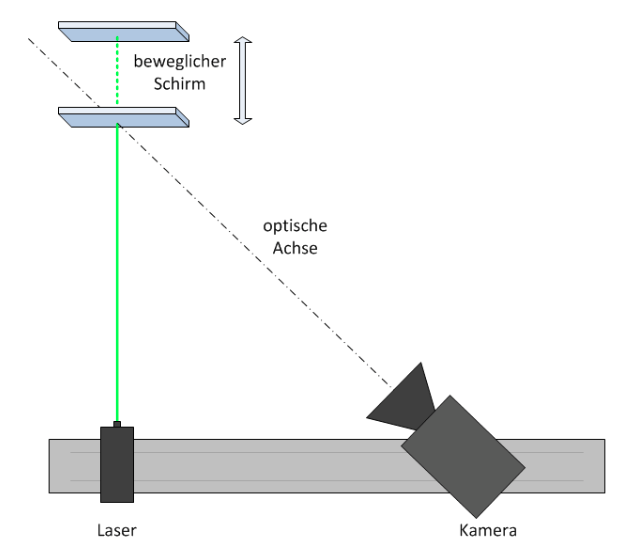
\includegraphics[width=0.8\linewidth]{img/Lasertriangulation_schema}
	\caption{Schematischer Versuchsaufbau \cite{versuchsanleitung_lasertriangulation}}
	\label{fig:schema_aufbau}
\end{figure}

\subsection{Herleitung}

In diesem Abschnitt erfolgt die Herleitung der Formel, durch die aus dem Abstand der Projektionen auf dem CCD-Sensor die Entfernungsänderung des Schirms berechnet werden kann. Die verwendeten Größen können Abbildung~\ref{fig:geometrie} entnommen werden.

Die zurückgelegte Entfernung ergibt sich aus der Differenz der Gesamtentfernung $z_{ges}$ und des Startpunktes $z_0$.
\begin{equation}
	z = z_{ges} - z_0
	\label{eq:z1}
\end{equation}
Da sich die Strahlengänge in rechtwinklige Dreiecke unterteilen lassen, können durch Anwendung des Cosinus- und Sinussatzes Ausdrücke für $z_{ges}$ und $z_0$ bestimmt werden, die nur von der Entfernung $d$ zwischen Linse und Laser und den Winkeln $\alpha$ und $\beta$ abhängen.
\begin{align}
	\left.\begin{aligned}
		\cos(\beta-\alpha) &= \frac{z_{ges}}{g'}\\
		\sin(\beta-\alpha) &= \frac{d}{g'}
	\end{aligned}\qquad\right\}\qquad z_{ges} &= d\cdot\frac{\cos(\beta-\alpha)}{\sin(\beta-\alpha)}\\[1em]
	\left.\begin{aligned}
		\cos(\beta) &= \frac{z_0}{g_1}\\ 
		\sin(\beta) &= \frac{d}{g_1}
	\end{aligned}\qquad\right\}\qquad z_0 &= d\cdot\frac{\cos(\beta)}{\sin(\beta)}
\end{align}
Die entstandenen Terme können nun in Gleichung~(\ref{eq:z1}) eingesetzt werden. Wie man leicht sieht lassen sich die Brüche der Winkelfunktionen in den Cotangens überführen. 
\begin{align}
	z &= d\cdot\left(\frac{\cos(\beta-\alpha)}{\sin(\beta-\alpha)}-\frac{\cos(\beta)}{\sin(\alpha)}\right)\\
	  &= d\cdot\left(\cot(\beta-\alpha)-\cot(\beta)\right)
	  \label{eq:z2}
\end{align}
Da der Winkel $\alpha$ nicht direkt gemessen werden kann muss ein Ausdruck gefunden werden, der von den Parametern des Optischen Systems abhängt. Dazu werden zunächst die Punktverschiebung auf dem CCD-Sensor $\Delta p'$ und die Bildweite $b$ als bekannt angenommen.
\begin{equation}
	\left.\begin{aligned}
		\sin(\alpha) &= \frac{\Delta p'}{b'}\\
	\cos(\alpha) &= \frac{b}{b'}
	\end{aligned}\qquad\right\}\qquad
	\frac{\sin(\alpha)}{\cos(\alpha)} = \frac{\Delta p'}{b} = \tan(\alpha)
\end{equation}
Durch Umkehrung des Tangens erhält man nun für $\alpha$:
\begin{equation}
	\alpha = \arctan\left(\frac{\Delta p'}{b}\right)
	\label{eq:alpha}
\end{equation}
Da auch der Abstand $d$ zwischen Brennpunkt und Laser nicht genau bestimmt werden kann, ist es notwendig diesen durch bekannte Größen zu substituieren. Abhilfe schafft hier die Anwendung des Sinussatzes auf den Winkel $\beta$.
\begin{align}
	\sin(\beta) &= \frac{d}{g_1}\\
	d &= g_1\cdot\sin(\beta)
	\label{eq:d}
\end{align}
Setzt man nun (\ref{eq:alpha}) und (\ref{eq:d}) in Gleichung~(\ref{eq:z2}) ein, so ergibt sich folgender Ausdruck:
\begin{equation}
	z = g_1\cdot\sin(\beta)\cdot\left\{\cot\left[\beta-\arctan\left(\frac{\Delta p'}{b}\right)\right]-\cot(\beta)\right\}
	\label{eq:z3}
\end{equation}
Mit Hilfe der Linsengleichung (\ref{eq:linsengleichung}) muss nun noch ein passender Ausdruck für $b$ gefunden werden.
\begin{align}
	\frac{1}{f} &= \frac{1}{b} + \frac{1}{g} \label{eq:linsengleichung}\\
	b &= \frac{f\cdot g}{g-f} \label{eq:b}
\end{align}
Durch das Einsetzen von (\ref{eq:b}) in Gleichung~(\ref{eq:z3}) ergibt sich ein Ausdruck für $z$, der nur von bekannten oder messbaren Größen abhängt. 
\begin{equation}
	z = g_1\cdot\sin(\beta)\cdot\left\{\cot\left[\beta-\arctan\left(\frac{\Delta p'(g-f)}{fg}\right)\right]-\cot(\beta)\right\}
	\label{eq:zfinal}
\end{equation}

\begin{figure}[h]
	\centering
	\begin{tikzpicture}[scale=0.8]
		% Linse zuerst, weil im Hintergrund
		\draw[fill=blue!15] (12,2) to[in=85,out=185] (8,-2) to[in=-95,out=5] (12,2) -- cycle;
		\draw[dashed] (12.5,2.5) node[anchor=west]{Hauptebene} -- (7.5,-2.5);
		% Grundgerüst
		\draw (0,0) -- (10,0) -- (10,3) coordinate (a3);
		% Laser
		\draw[green!90!black, thick] (0,0) -- (0,10);
		\draw[red, thick, dashed] (0,10) -- (0,12);
		% gestrichelte Linie
		\draw[dash dot] (12.5,-2.5) coordinate (a6) -- (10,0);
		\draw[dash dot] (10,0) coordinate (a2) -- (0,10) coordinate (a1);
		\draw[dash dot]	(0,10) -- (-1,11);
		% blau gestrichelte Linie
		\draw[dash dot, blue] (10,0) -- (0,12) coordinate (a4);
		\draw[dash dot, blue] (12.27,-2.72) coordinate (a7) -- (10,0);
		% Sensor und Schärfeebene
		\draw (-1,11) coordinate (a5) -- (0,12);
		\draw (11.5,-3.5) -- (13.5,-1.5);
		% Winkelbezeichnungen
		\draw pic["$\beta$", draw=black, angle eccentricity=0.8, angle radius=2cm]{angle=a3--a2--a1};
		\draw pic["$\alpha$", draw=black, angle eccentricity=0.95, angle radius=7cm]{angle=a4--a2--a1};
		\draw pic["$\cdot$", draw=black, angle eccentricity=0.5, angle radius=0.3cm]{angle=a1--a5--a4};	
		\draw pic["$\cdot$", draw=black, angle eccentricity=0.5, angle radius=0.2cm]{angle=a2--a6--a7};
		% Beschriftungen
		\draw (5,5) node[anchor=north east]{$g_1$};
		\draw (-0.5,10.5) node[anchor=north east]{$g_2$};
		\draw (0,11) node[anchor=west, red]{$z$};
		\draw (-0.5,11.5) node[anchor=south east]{$\Delta p$};
		\draw (5,6) node [anchor=south west, blue]{$g'$};
		\draw (11.25,-1.25) node [anchor=south west]{$b$};
		\draw (11.1,-1.4) node [anchor=north east, blue]{$b'$};
		\draw (12.4,-2.6) node [anchor=north west]{$\Delta p'$};
		\draw (13.5,-1.5) node [anchor=west]{CCD-Sensor};
		\draw (0,5) node[anchor=west, green!90!black]{$z_0$};
	\end{tikzpicture}
	\caption{Geometrische Darstellung der Strahlengänge}
	\label{fig:geometrie}
\end{figure}